\newpage

\section{Diseño conceptual}
\label{sec:diseno-conceptual}

En esta sección se presenta el diseño conceptual de la base de datos, que se construyó en dos momentos: un modelo entidad-relación básico, elaborado a partir de la entrevista en la Práctica~1, y su versión extendida, elaborada en la Práctica~2 para representar las reglas que el modelo básico no podía expresar.

\subsection{Modelo entidad-relación inicial}

El primer modelo identificó los objetos del negocio sobre los cuales el salón necesita guardar información: el evento, la mesa, la cuenta de cada grupo de invitados, la comanda, el producto, el ingrediente, el pago, el anticipo, el paquete contratado y el usuario que opera el sistema. Cada uno se definió como entidad porque tiene datos propios y participa en reglas de la operación, y cada asociación que el cliente describió se representó como una relación con su razón de cardinalidad. La Figura~\ref{fig:diagrama-er} muestra el diagrama resultante.

En este modelo, la comanda ocupa el lugar central: sustituye a la comanda de papel, se liga a la cuenta que la generó, al producto que se pidió y al personal que la atendió, y registra su estado. Separar la cuenta de la mesa permite cobrar por grupo de invitados, y separar el anticipo del pago distingue los depósitos del organizador, ligados al evento, de los cobros que se hacen a cada cuenta durante el evento.

\begin{paginahorizontal}
    \vspace*{\fill}
    \begin{figure}[H]
        \centering
        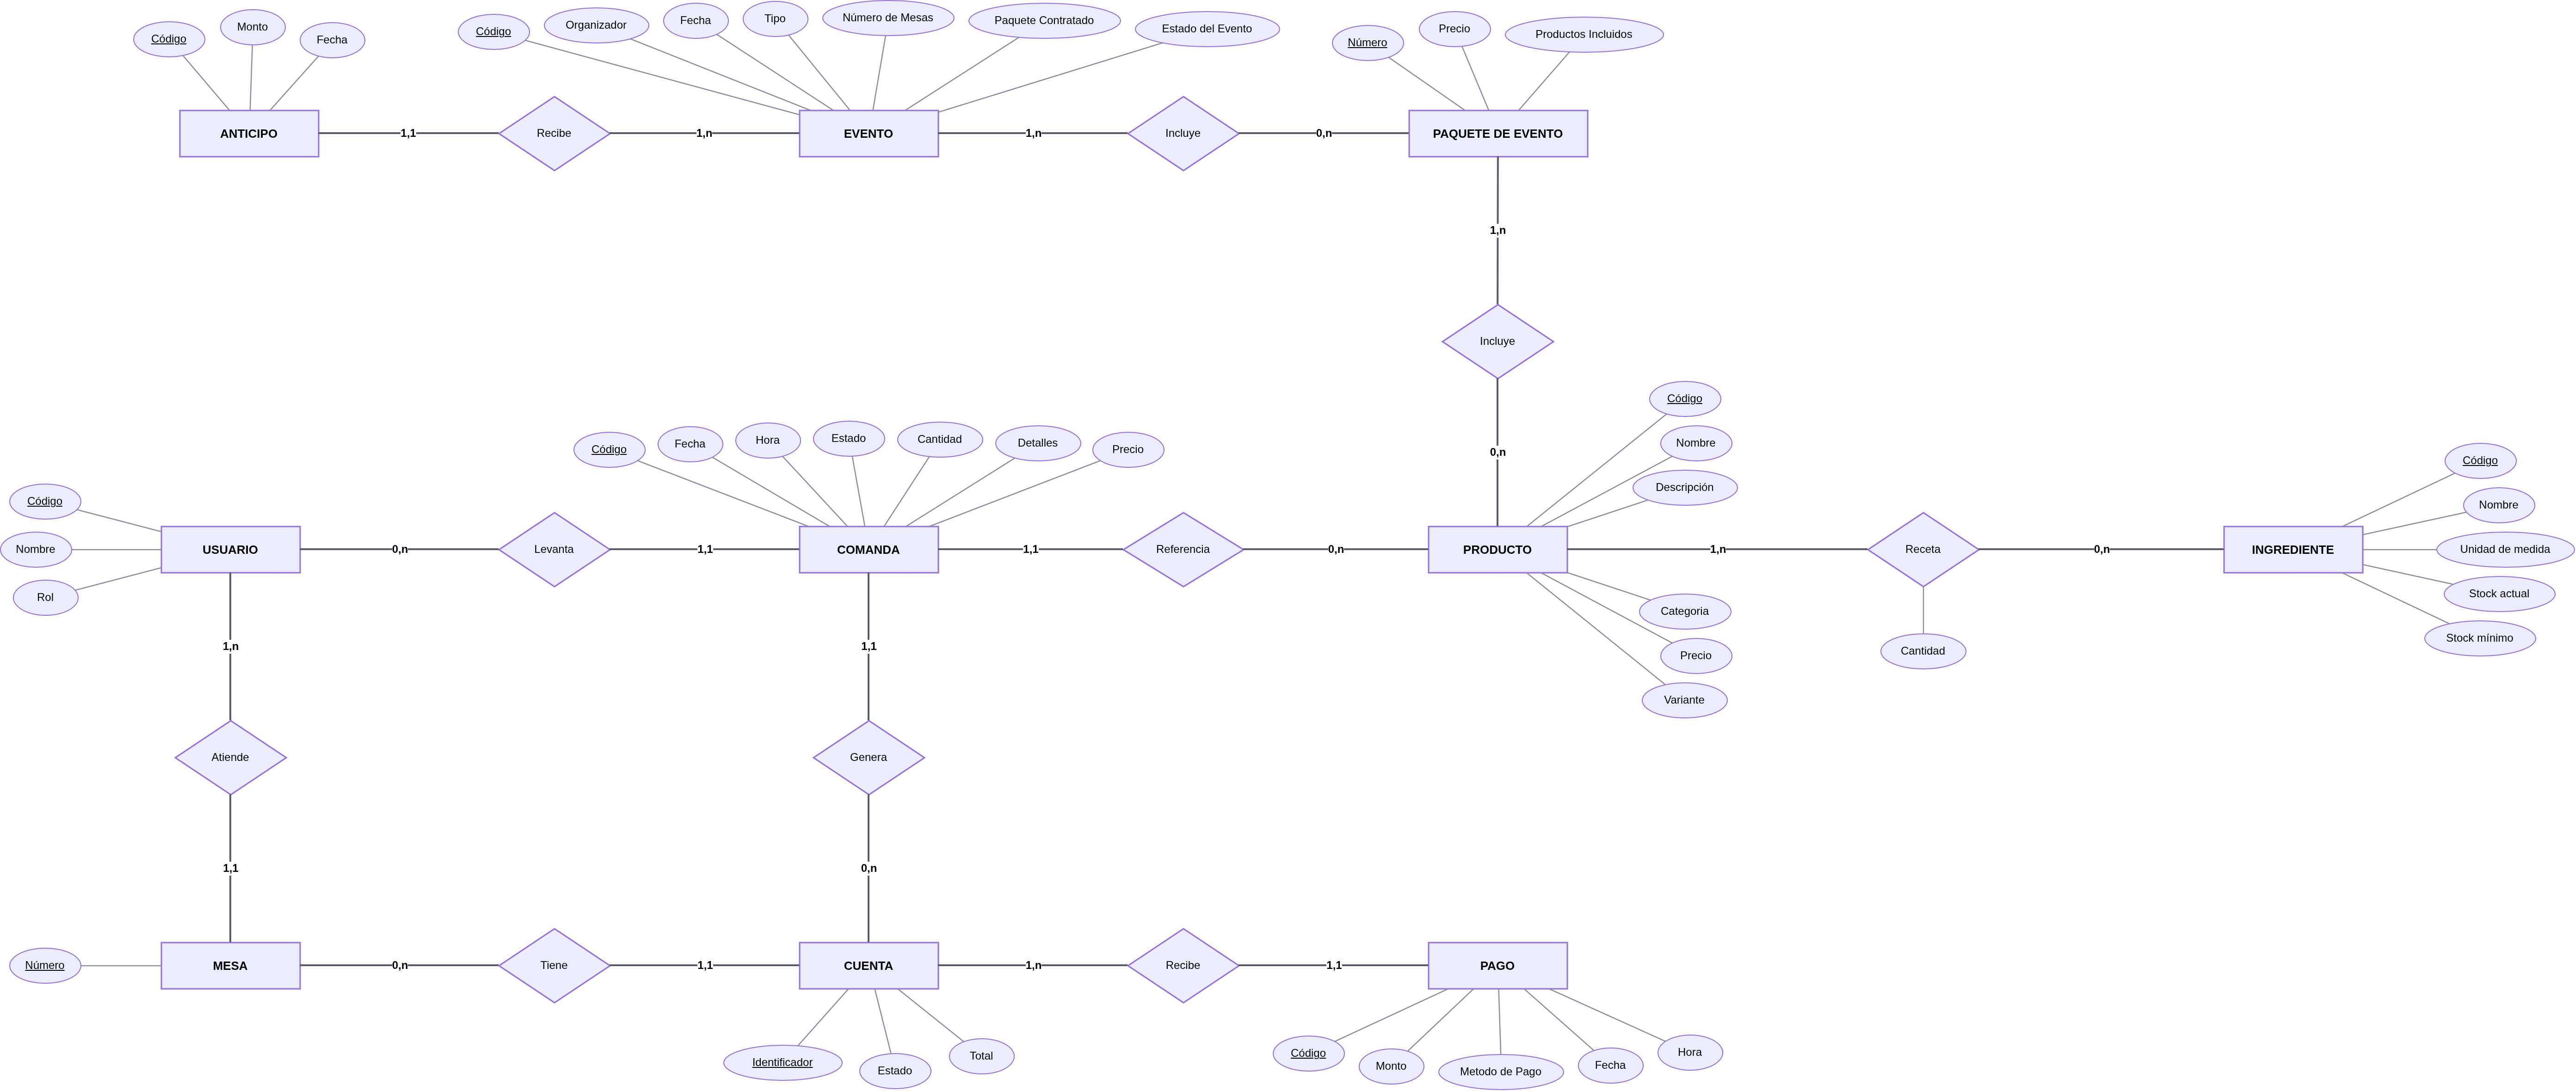
\includegraphics[width=\linewidth, height=0.8\textheight, keepaspectratio]{../../modelo/diagrama-er.png}
        \captionsetup{labelfont=bf, textfont=it, labelsep=newline, justification=raggedright, singlelinecheck=false}
        \caption{Diagrama entidad-relación inicial}
        \label{fig:diagrama-er}
    \end{figure}
    \vspace*{\fill}
\end{paginahorizontal}

\subsection{Limitaciones del modelo básico}

Al revisar de nuevo la entrevista en la Práctica~2, se encontró que el modelo básico obligaba a aplanar o a omitir varias reglas que el cliente sí había mencionado. La Tabla~\ref{tab:er-a-eer} resume esas reglas y el concepto del modelo extendido con el que se representaron.

\begin{table}[H]
    \centering
    \small
    \begin{tabularx}{\textwidth}
        {
            >{\RaggedRight\arraybackslash}X
            >{\RaggedRight\arraybackslash}p{4.2cm}
            >{\RaggedRight\arraybackslash}p{4.2cm}
        }
        \toprule
        \textbf{Regla del negocio} & \textbf{Modelo básico} & \textbf{Modelo extendido} \\
        \midrule
        Los números de mesa y de cuenta se reinician en cada evento. & Mesa y Cuenta con clave propia. & Entidades débiles identificadas por el evento. \\
        Meseros, cocina y bar, y caja guardan datos distintos y realizan funciones distintas. & Un atributo \textit{rol} en Usuario. & Jerarquía de especialización de Usuario. \\
        Ninguna mesa queda sin mesero, pero un mesero puede no tener mesas. & Razón 1:N, sin indicar la obligatoriedad. & Cardinalidades $(\mathit{min}, \mathit{max})$. \\
        Lo acordado de cada producto cambia de un evento a otro aunque sea el mismo paquete. & Solo el contenido general del paquete. & Relación ternaria \textit{Acuerda} con su cantidad. \\
        Un evento puede tener varios organizadores. & Un solo valor por atributo. & Atributo multivaluado. \\
        La fecha y la hora se consultan por día, mes y año. & Campos sueltos. & Atributos compuestos. \\
        \bottomrule
    \end{tabularx}
    \captionsetup{labelfont=bf, textfont=it, labelsep=newline, justification=raggedright, singlelinecheck=false}
    \caption{Reglas que motivaron el modelo extendido}
    \label{tab:er-a-eer}
\end{table}

\subsection{Modelo entidad-relación extendido}

El modelo extendido conserva las entidades del modelo inicial y les agrega los conceptos de la Tabla~\ref{tab:er-a-eer}. Se representó en la notación de Peter Chen, en la que las entidades se dibujan como rectángulos, las relaciones como rombos y los atributos como óvalos; las entidades débiles y sus relaciones identificadoras se distinguen con doble contorno. La Figura~\ref{fig:diagrama-eer} muestra el diagrama completo.

\begin{paginahorizontal}
    \vspace*{\fill}
    \begin{figure}[H]
        \centering
        \includegraphics[width=\linewidth, height=0.8\textheight, keepaspectratio]{../../modelo/diagrama-eer-chen.png}
        \captionsetup{labelfont=bf, textfont=it, labelsep=newline, justification=raggedright, singlelinecheck=false}
        \caption{Diagrama entidad-relación extendido en notación de Peter Chen}
        \label{fig:diagrama-eer}
    \end{figure}
    \vspace*{\fill}
\end{paginahorizontal}

\subsubsection{Entidades débiles}

Mesa y Cuenta son entidades débiles con dependencia de identificación respecto del evento, como se resume en la Tabla~\ref{tab:entidades-debiles}. Decir \enquote{la mesa tres} o \enquote{la cuenta diez} no identifica nada si no se indica el evento, porque la numeración se reinicia en cada uno. Por la misma razón, ninguna de las dos puede existir sin el evento al que pertenece.

\begin{table}[H]
    \centering
    \small
    \begin{tabularx}{\textwidth}
        {
            >{\RaggedRight\arraybackslash}p{2.2cm}
            >{\RaggedRight\arraybackslash}p{2.6cm}
            >{\RaggedRight\arraybackslash}p{3cm}
            >{\RaggedRight\arraybackslash}X
        }
        \toprule
        \textbf{Entidad débil} & \textbf{Propietaria} & \textbf{Clave parcial} & \textbf{Clave completa} \\
        \midrule
        Mesa & Evento & Número de mesa & (Número de evento, Número de mesa) \\
        Cuenta & Evento & Secuencial & (Número de evento, Secuencial) \\
        \bottomrule
    \end{tabularx}
    \captionsetup{labelfont=bf, textfont=it, labelsep=newline, justification=raggedright, singlelinecheck=false}
    \caption{Entidades débiles del modelo}
    \label{tab:entidades-debiles}
\end{table}

\subsubsection{Jerarquía de Usuario}

Usuario se especializa en tres subclases: Mesero, Bar/Cocina y Cajero/Administrador. La especialización se justifica porque cada subclase tiene atributos propios, como el turno del mesero o la estación asignada de la cocina o el bar, y sobre todo relaciones propias: el mesero atiende mesas y levanta comandas, la cocina y el bar preparan comandas, y el cajero maneja pagos y cancela comandas. Si solo cambiaran los atributos, un campo de rol habría bastado.

La especialización es \textbf{disjunta}, porque una persona desempeña un solo puesto a la vez, y esa separación es la que da sentido al control que pidió el cliente: quien cobra no puede ser quien recibe la propina de ese cobro, y quien cancela una comanda no puede ser quien la levantó. Es además \textbf{total}, porque todo usuario del sistema es personal del salón y tiene un puesto; el organizador del evento no es usuario, sino un dato del evento. La cocina y el bar se agruparon en una sola subclase porque tienen los mismos atributos y la misma función, y su estación asignada indica cuál es cuál.

\subsubsection{Relaciones y cardinalidades}

Las cardinalidades se expresaron con la notación $(\mathit{min}, \mathit{max})$, que indica para cada entidad con cuántas instancias de la otra se asocia como mínimo y como máximo. La Tabla~\ref{tab:relaciones} reúne las diecisiete relaciones del modelo; en cada par, la primera cardinalidad corresponde a la primera entidad.

\begin{table}[H]
    \centering
    \footnotesize
    \begin{tabularx}{\textwidth}
        {
            >{\RaggedRight\arraybackslash}p{3.2cm}
            >{\RaggedRight\arraybackslash}p{4.6cm}
            >{\RaggedRight\arraybackslash}p{2.4cm}
            >{\RaggedRight\arraybackslash}X
        }
        \toprule
        \textbf{Relación} & \textbf{Entidades} & \textbf{Cardinalidad} & \textbf{Regla} \\
        \midrule
        \textit{Pertenece} (identificadora) & Mesa -- Evento & (1,1):(1,N) & Toda mesa es de un evento y todo evento tiene mesas. \\
        \textit{Abre} (identificadora) & Evento -- Cuenta & (0,N):(1,1) & Toda cuenta se abre en un evento. \\
        \textit{Atiende} & Mesa -- Mesero & (1,1):(0,N) & Ninguna mesa queda sin mesero. \\
        \textit{Tiene} & Mesa -- Cuenta & (0,N):(1,1) & Una mesa tiene varias cuentas. \\
        \textit{Genera} & Cuenta -- Comanda & (0,N):(1,1) & Una cuenta pide varias rondas. \\
        \textit{Levanta} & Mesero -- Comanda & (0,N):(1,1) & Cada comanda tiene un mesero responsable. \\
        \textit{Prepara} & Bar/Cocina -- Comanda & (0,N):(0,1) & Una comanda pendiente aún no tiene estación. \\
        \textit{Cancela} & Cajero -- Comanda & (0,N):(0,1) & Solo caja cancela comandas. \\
        \textit{Referencia} & Comanda -- Producto & (1,1):(0,N) & Cada comanda pide un producto. \\
        \textit{Variante} & Producto -- Producto & (0,N):(0,1) & Una variante tiene un solo producto principal. \\
        \textit{Receta} & Producto -- Ingrediente & (1,N):(0,N) & Todo producto lleva al menos un ingrediente. \\
        \textit{Incluye} & Paquete -- Producto & (1,N):(0,N) & Contenido base de cada paquete. \\
        \textit{Acuerda} (ternaria) & Evento -- Paquete -- Producto & (0,N) en cada una & Lo pactado para cada evento. \\
        \textit{Recibe} & Evento -- Anticipo & (0,N):(1,1) & Los anticipos son del evento. \\
        \textit{Recibe} & Cuenta -- Pago & (0,N):(1,1) & Una cuenta puede pagarse en partes. \\
        \textit{Maneja} & Cajero -- Pago & (0,N):(1,1) & Cada pago lo registra un cajero. \\
        \textit{Recibe propina} & Mesero -- Pago & (0,N):(0,1) & Un pago puede dejar propina a un mesero. \\
        \bottomrule
    \end{tabularx}
    \captionsetup{labelfont=bf, textfont=it, labelsep=newline, justification=raggedright, singlelinecheck=false}
    \caption{Relaciones del modelo entidad-relación extendido}
    \label{tab:relaciones}
\end{table}

\subsubsection{Relación ternaria y atributos de relación}

Una relación entre tres entidades solo se justifica cuando ninguna de ellas queda determinada por las otras dos. \textit{Acuerda} cumple esa condición: si un evento contrata dos paquetes que incluyen el mismo producto, conocer el evento y el producto no indica cuánto se acordó por cada paquete, por lo que se necesitan las tres entidades. En cambio, \textit{Prepara} se mantuvo binaria, porque cada comanda apunta a un solo producto y agregarlo a la relación no aportaba información.

Tres datos no pertenecen a ninguna entidad, sino a la relación que las une: la \textit{cantidad acordada} de \textit{Acuerda}, base de la comparación entre lo presupuestado y lo consumido; la \textit{cantidad por porción} de \textit{Receta}, con la que se descuenta el inventario al preparar cada comanda; y el \textit{monto de propina} de \textit{Recibe propina}, que corresponde a un cobro concreto y no al mesero ni al pago por separado.

\subsubsection{Atributos especiales}

El modelo incluye un atributo multivaluado, los organizadores del evento, y atributos compuestos para la fecha y la hora, que se consultan por sus componentes. También identifica atributos derivados, cuyo valor se calcula a partir de otros datos y no se captura: el total acumulado de cada cuenta, las propinas acumuladas de cada mesero, la edad de cada usuario, el número de mesas de cada evento y la disponibilidad de cada producto, que depende de que todos los ingredientes de su receta alcancen para una porción.

\subsection{Restricciones que el diagrama no expresa}

Un diagrama entidad-relación no puede representar todas las reglas del negocio. Las siguientes quedaron documentadas junto al modelo para resolverse en la implementación:

\begin{itemize}
    \item El total acumulado de una cuenta debe coincidir con la suma de sus comandas.
    \item El precio cobrado se copia del catálogo al levantar la comanda y no cambia aunque después cambie el precio del producto.
    \item Solo el cajero o administrador puede cancelar comandas.
    \item Al preparar una comanda se descuenta del inventario la cantidad por porción de cada ingrediente, y la existencia nunca puede quedar negativa.
    \item El rol que se guarda es el actual: si un mesero pasa a caja, las comandas y los pagos que ya registró conservan su autoría.
    \item El contenido de un paquete es una base y no una lista cerrada, por lo que en un evento pueden acordarse productos o cantidades distintos de los del catálogo.
\end{itemize}

La sección de implementación describe cómo cada una de estas reglas se convirtió en una restricción, un disparador o una vista del esquema.
